\documentclass{article}
\usepackage[T2A]{fontenc}
\usepackage[utf8x]{inputenc}
\usepackage[english, ukrainian]{babel}
\usepackage{url}
\usepackage{latexsym,amsmath,amsfonts,amssymb,amsthm,mathrsfs}
\usepackage{cite,hhline}
\usepackage{hyperref}
\usepackage{graphicx,mwe}
\usepackage{wrapfig}
\usepackage{array}
\usepackage{tabularx, multirow}
\usepackage{longtable}
\usepackage{lipsum} % just for dummy text- not needed for a longtable

\addto\captionsukrainian{\renewcommand{\figurename}{Мал.}}
\usepackage{book}					% стильовий файл журналу 

\title{Мій перший документ}
\date{2022-11-14}
\author{МАН }



\begin{document}
	\maketitle
	\newpage
	
\Title{Оформлення шаблону книги}\label{radap1xxx:FirstPage}
\Authors{Мосійчук В.С.}
\aff{Київський політехнічний інститут імені Ігоря Сікорського, м. Київ, Україна}
\Address{}{\href{mailto:mvs@ros.kpi.ua}{mvs@ros.kpi.ua}}
\AbsKeywords{У роботі представлені вимоги щодо оформлення статей для подання у збірник наукових праць ``Вісник Національного технічного університету України <<Київський політехнічний інститут>>. Серія Радіотехніка. Радіоапаратобудування''. Показано, що дотримання встановлених правил дозволить покращити вашу статтю .
}{Ключові слова}{правила оформлення, радіотехніка, радіоапаратобудування, \LaTeX}
	


	
\section{Тест підтримки української мови}
	
Obviously the statements title, date and author are not within the the document environment, so they will not directly show up in our document. The area before our main document is called preamble. In this specific example we use it to set up the values for the maketitle command for later use in our document. This command will automagically create a titlepage for us. The newpage command speaks for itself.

If we now compile again, we will see a nicely formatted title page, but we can spot a page number at the bottom of our title page. What if we decide, that actually, we don’t want to have that page number showing up there. We can remove it, by telling LaTeX to hide the page number for our first page. This can be done by adding the pagenumbering{gobble} command and then changing it back to \pagenumbering{arabic} on the next page numbers like so:

%Привіт світ

Формула кола: $ y^2 + x^2 = 1  $
$$
 y = \sqrt{x+1}
$$

\[
y = \sqrt{x^2+1}
\]


\begin{equation}\label{eq1}
	H(A)=-\sum \limits_{i=1}^n p_i \log p(p_i)
\end{equation}

\begin{equation}\label{eq2}
	H(A)=-\sum \limits_{i=1}^n p_i 
\end{equation}

That’s it. You’ve successfully created your first LaTeX document. The following lessons will cover how to structure your document and we will then proceed to make use of many features of LaTeX.

\subsection{Begin subsection}
Obviously the statements title, date and author are not within the the document environment, so they will not directly show up in our document. The area before our main document is called preamble. In this specific example we use it to set up the values for the maketitle command for later use in our document. This command will automagically create a titlepage for us. The newpage command speaks for itself.

\begin{wrapfigure}{L}{0.5\textwidth}
%\begin{figure}[htp]
	\raggedleft %note: there's going to be another image next to this later
	\includegraphics[width=5cm]{example-image-a}\\
	\noindent
	- Point 1 under the first description\\
	\caption{\label{fig:frog1} Підпис до рисунку.}
\end{wrapfigure} 
If we now compile again, we will see a nicely formatted title page, but we can spot a page number at the bottom of our title page. What if we decide, that actually, we don’t want to have that page number showing up there. We can remove it, by telling LaTeX to hide the page number for our first page. This can be done by adding the pagenumbering{gobble} command and then changing it back to \pagenumbering{arabic} on the next page numbers like so:

\begin{wrapfigure}{R}{0.4\textwidth}
	\raggedright
	\includegraphics[width=0.38\textwidth]{example-image-b}\\
	\caption{\label{fig:frog2} Підпис до рисунку.}
\end{wrapfigure}
If we now compile again, we will see a nicely formatted title page (Мал. \ref{fig:frog1}), but we can spot a page number at the bottom of our title page. What if we decide, that actually, we don’t want to have that page number showing up there. We can remove it, by telling LaTeX to hide the page number for our first page. This can be done by adding the pagenumbering{gobble} command and then changing it back to \pagenumbering{arabic} on the next page numbers like so:
If we now compile again, we will see a nicely formatted title page, but we can spot a page number at the bottom of our title page. What if we decide, that actually, we don’t want to have that page number showing up there. We can remove it, by telling LaTeX to hide the page number for our first page. This can be done by adding the pagenumbering{gobble} command and then changing it back to \pagenumbering{arabic} on the next page numbers like so:


If we now compile again, we will see a nicely formatted title page, but we can spot a page number at the bottom of our title page. What if we decide, that actually, we don’t want to have that page number showing up there. We can remove it, by telling LaTeX to hide the page number for our first page. This can be done by adding the pagenumbering{gobble} command and then changing it back to \pagenumbering{arabic} on the next page numbers like so:


	
\section{Таблиці}
	
Obviously the statements title, date and author are not within the the document environment, so they will not directly show up in our document. The area before our main document is called preamble. In this specific example we use it to set up the values for the maketitle command for later use in our document. This command will automagically create a titlepage for us. The newpage command speaks for itself.

If we now compile again, we will see a nicely formatted title page, but we can spot a page number at the bottom of our title page. What if we decide, that actually, we don’t want to have that page number showing up there. We can remove it, by telling LaTeX to hide the page number for our first page. This can be done by adding the pagenumbering{gobble} command and then changing it back to \pagenumbering{arabic} on the next page numbers like so:




\section{Висновки}

A document has a preamble and document part
The document environment must be defined
\begin{itemize}
	\item Commands beginning with a backslash \, environments have a begin and end tag
	\item Useful settings for pagenumbering:
	\item gobble – no numbers
	\item arabic – arabic numbers
	\item roman – roman numbers
	\item roman – roman numbers2
	\item roman – roman numbers3
	\item roman – roman numbers4
	\item roman – roman numbers5
\end{itemize}


\section {Копище- Лозко Валерій}
\begin{center}
	\begin{tabular}{| l | c |}
		\hline
		Засноване  & 1459 р.\\ 
		\hline
		Населення & 983 \\ 
		\hline 
		Площа & 2,83 км² \\   
		\hline
	\end{tabular}
\end{center}

\subsection{Історія села Копище}

Копище — село розташоване на березі річки Уборті (притока Прип’яті), за 55 км від районного центру та залізничної станції Олевськ.

Після Андрусівського перемир’я 1667 року село залишилося у складі Польщі. Боротьбу проти своїх поневолювачів селяни не припиняли. Вони активно боролися під час визвольного повстанського руху проти польсько-шляхетських загарбників’ за возз’єднання Правобережної України з Росією під проводом С. Палія у кінці XVII — на початку XVIII століття.

Страшних бідувань зазнали селяни Копища в раки першої світової війни. Відчувалася нестача робочих рук, тягла, скоротилися посівні площі, голод і хвороби косили людей.

Звістку про Лютневу буржуазно-демократичну революцію 1917 року в село принесли солдати, які поверталися з фронту. Всі чекали змін у житті, вимагали розподілу земель, але Тимчасовий уряд не поспішав поліпшувати становище трудового народу.

Активними борцями за нове життя були копищанські жінки. Так, у постійно діючих комісіях при сільраді їх працювало 4, у комнезамі — 3, у касі взаємодопомоги — 3, у шкільній раді — 3, у правлінні кредитного товариства — 3. На з’їзд жінок Олевського району 1925 року від Конища поїхало 16 жінок.

1927 року в селі Копищі було організовано перше колективне господарство — ТСОЗ, що охопив спершу 12 господарств, а на початку 1928 року — вже 35. Товариство мало всього лише 8 коней, 4 плуги, 4 борони, 2 культиватори та сівалку. В перші місяці його існування держава надала кредити в розмірі 7690 крб. на будівництво господарчих приміщень, придбання робочої худоби, на закладення саду.

1936 року в селі діяли медична амбулаторія, пологовий будинок на 8 ліжок, де, крім лікаря, працювали дві акушерки та дві санітарки. Під час жнив відкривалися дитячі ясла на 120 місць.

1936 року збудовано нове приміщення семирічної школи, де 8 учителів навчали 300 учнів. Добра слава йшла про роботу Копищанського клубу. Тут читалися лекції й доповіді. У залі на 200 місць ставилися концерти силами гуртківців, двічі на місяць демонструвалися кінокартини. Сільська бібліотека мала книжковий фонд 6 тис. примірників. Товарами народного споживання трудящих забезпечували два магазини.

13 липня 1941 року в село (вдерлися фашисти. Настали чорні дні неволі. Гітлерівці грабували населення, забирали хліб, худобу. 70 мирних жителів вивезли на каторжні роботи до Німеччини.

13 липня 1943 року в с.Копище сталася одна з найжахливіших трагедій України: нацистські загарбники влаштували каральну операцію “Фрау Хельга” (пані Ольга), метою якої було повне знищення жителів села. За один день спалили живими 2887 мирних жителів, з них 1347 дітей віком до 12 років. Врятувались лише четверо дорослих та 46 дітей.
\begin{figure}[h]
	
	\centering
	
	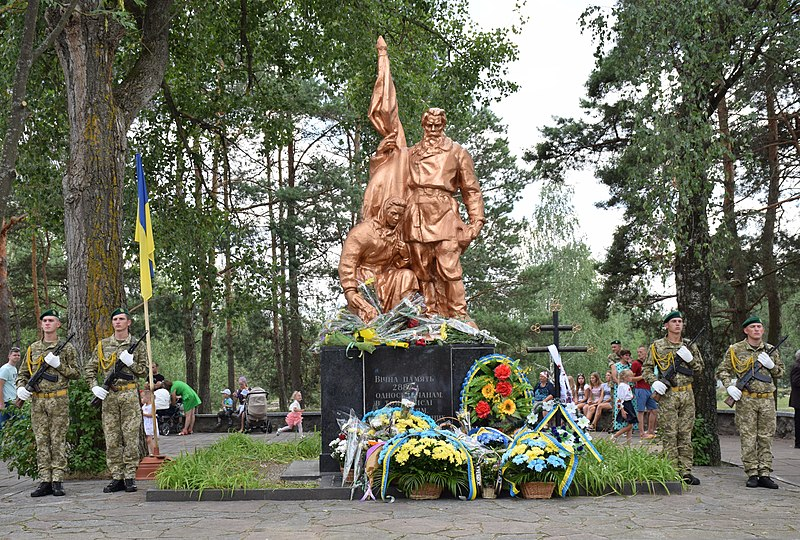
\includegraphics[width=0.8\linewidth]{0.jpg}
	
	\caption{Пам'ятник односельцям, загиблим в результаті трагедії 13 липня 1943 р.}
	
	\label{fig:mpr}
	
\end{figure}
Незважаючи на величезні труднощі, копищанці всі сили віддавали на відродження рідного села. Стало легше працювати, коли після перемоги над гітлерівською Німеччиною до села почали повертатися демобілізовані чоловіки.

Поступово піднімалося з руїн Копище. Вже через рік після перемоги тут виросла ціла вулиця. Один з будинків пристосували під лікарняний пункт, інший під початкову школу.

Основні сільськогосподарські культури у колгоспі — льон, картопля, зернові. Важливу роль у його економіці відіграє тваринництво м’ясо-молочного напряму. На 1 січня 1967 року колгосп мав 685 голів великої рогатої худоби, в т. ч. 275 корів та 199 голів овець. Для їх розміщення споруджено під шифером 5 добротних тваринницьких приміщень. На той час господарство було повністю електрифіковано, мало 9 тракторів, 6 комбайнів, 8 автомашин. Діяла пилорама.

На тваринницьких фермах обладнано автоматичне напування.

Копищанці справжні господарі своєї долі. 35 чоловік обрано депутатами сільської Ради, серед яких 15 жінок, 11 чоловік — членами правління колгоспу. В постійно діючих комісіях працює близько 100 чоловік. Бюджет Ради на 1973 рік становить 39 964 крб., переважна більшість цієї суми буде використана на поліпшення охорони здоров’я, на піднесення культурно-освітньої роботи.

В центрі Копища знаходиться Братьска могила жертвам фатишизму (1961 р.), в якій поховано 2887 жителів села, утому числі 1347 дітей.
\begin{figure}
	\centering
	\begin{subfigure}[b]{0.3\textwidth}
		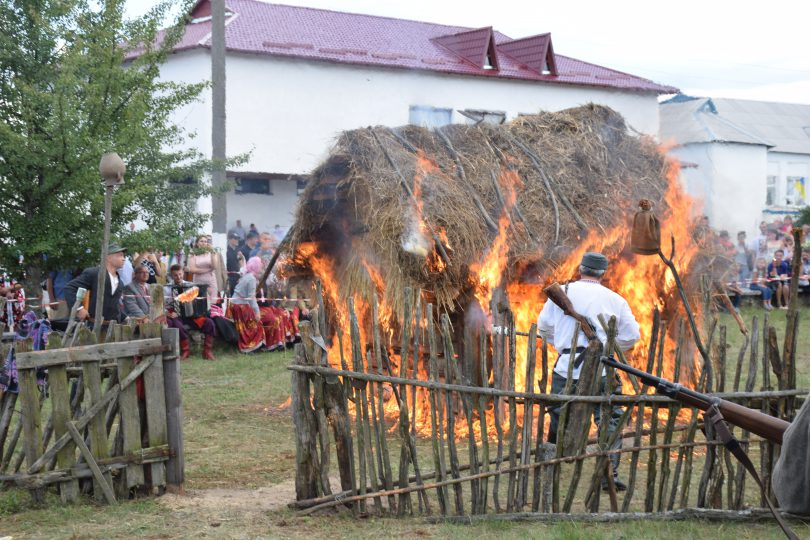
\includegraphics[width=\textwidth]{1.jpg}
		\caption{}
		\label{fig:gull}
	\end{subfigure}
	~ %add desired spacing between images, e. g. ~, \quad, \qquad, \hfill etc. 
	%(or a blank line to force the subfigure onto a new line)
	\begin{subfigure}[b]{0.3\textwidth}
		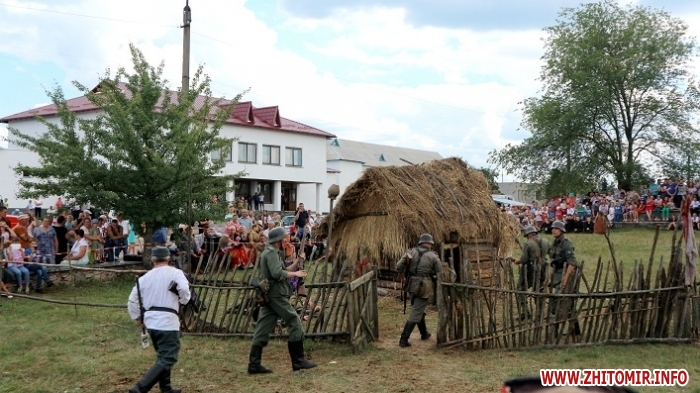
\includegraphics[width=\textwidth]{2.jpg}
		\caption{}
		\label{fig:tiger}
	\end{subfigure}
	~ %add desired spacing between images, e. g. ~, \quad, \qquad, \hfill etc. 
	%(or a blank line to force the subfigure onto a new line)
	\begin{subfigure}[b]{0.3\textwidth}
		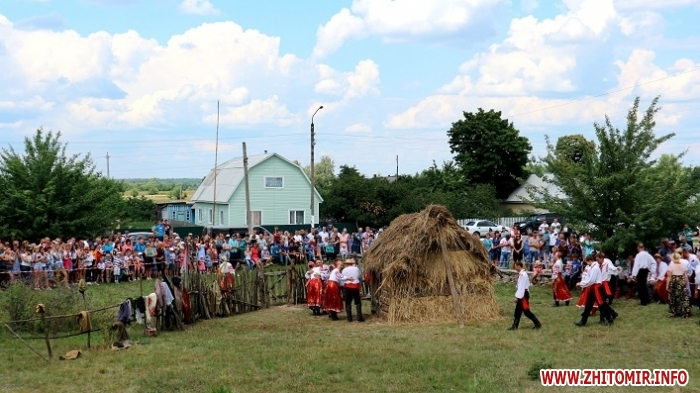
\includegraphics[width=\textwidth]{3.jpg}
		\caption{}
		\label{fig:mouse}
		\end{subfigure}
	\caption{Відзначення 75-ї річниці Копищенської трагедії}\label{fig:animals}
\end{figure}
\begin{figure}[h]
	
	\centering
	
	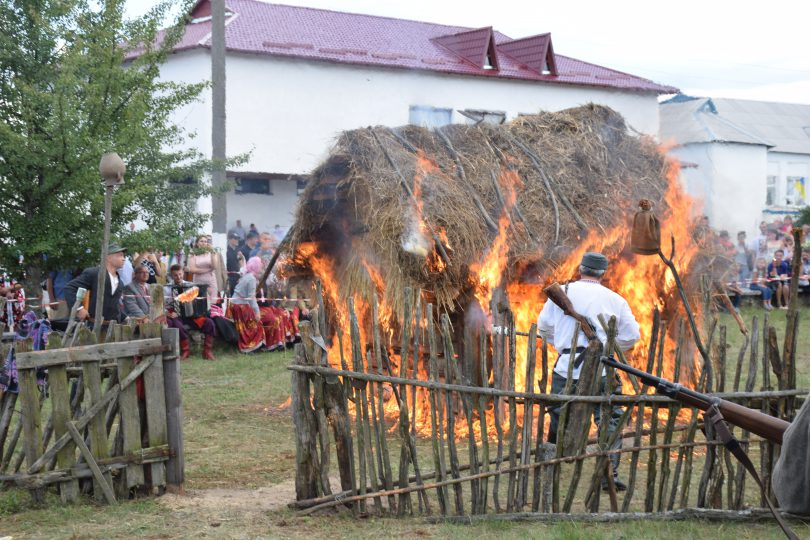
\includegraphics[width=0.8\linewidth]{1.jpg}
	
	\caption{Відзначення 75-ї річниці Копищенської трагедії}
	
	\label{fig:mpr}
	
\end{figure}
Поруч знаходиться музей, який розповідає людям про історію рідного села і про страшну трагедію, яку не можна забути. Директор музею – Мартиновець Марія Василівна.

У селі наразі є загальноосвітня школа І-ІІІ ступенів. Директор – Лозко Марія Михайлівна. Дітей навчається 186. Також функціонує заклад дошкільної освіти з короткотривалим перебуванням дітей без харчування, який відвідує 22 дітей.







\end{document}
